\chapter{Introduzione alla Programmazione Concorrente}

\section{Salto dei ranocchi}


\begin{figure}[h]
    \centering
    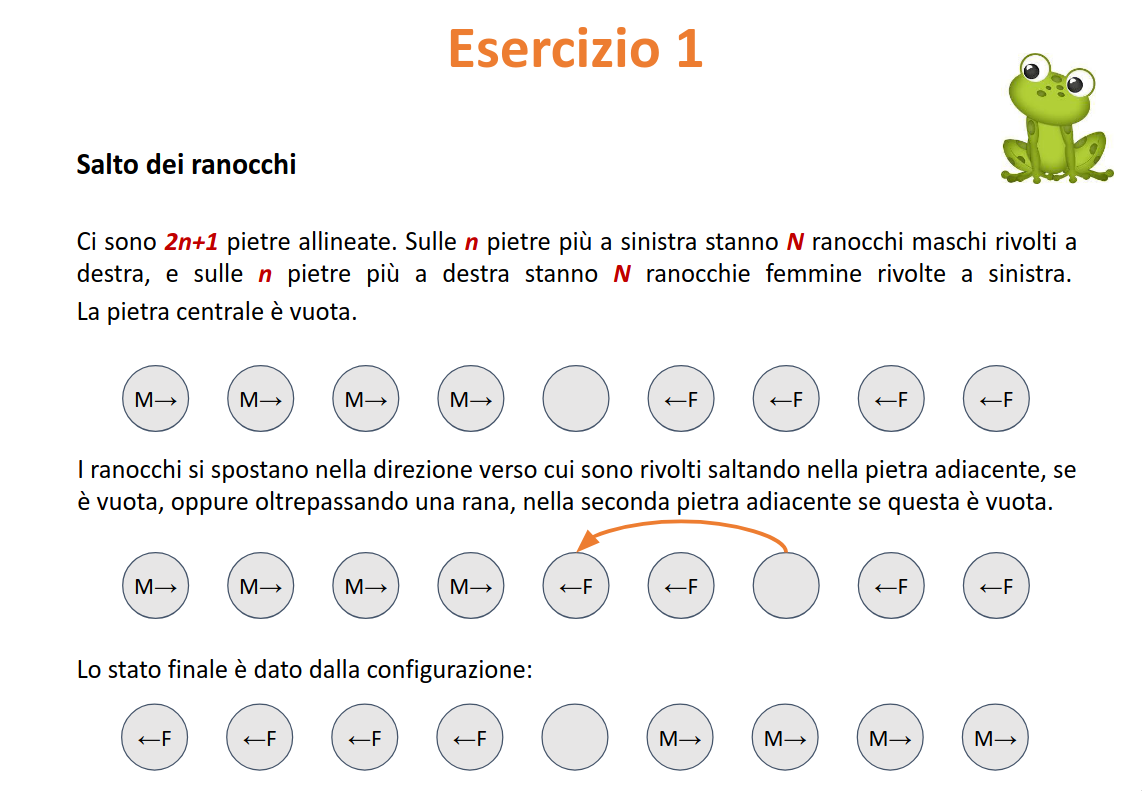
\includegraphics[scale=0.35]{01-IntroduzioneAllaProgrammazioneConcorrente/1-1.png}
\end{figure}

\subsubsection{Si consideri il diagramma degli stati per n = 1 e per n = 2 e, per entrambi i casi, si risponda alle seguenti domande:}

\begin{enumerate}
  \item [a.] esiste una computazione che, partendo dallo stato iniziale porti allo stato finale?
  \item [b.] tutte le computazioni raggiungono lo stato finale?
  \item [c.] esistono computazioni che non terminano, cioè non raggiungono uno stato in cui non si può eseguire nessuna mossa?
\end{enumerate}

\begin{center}
    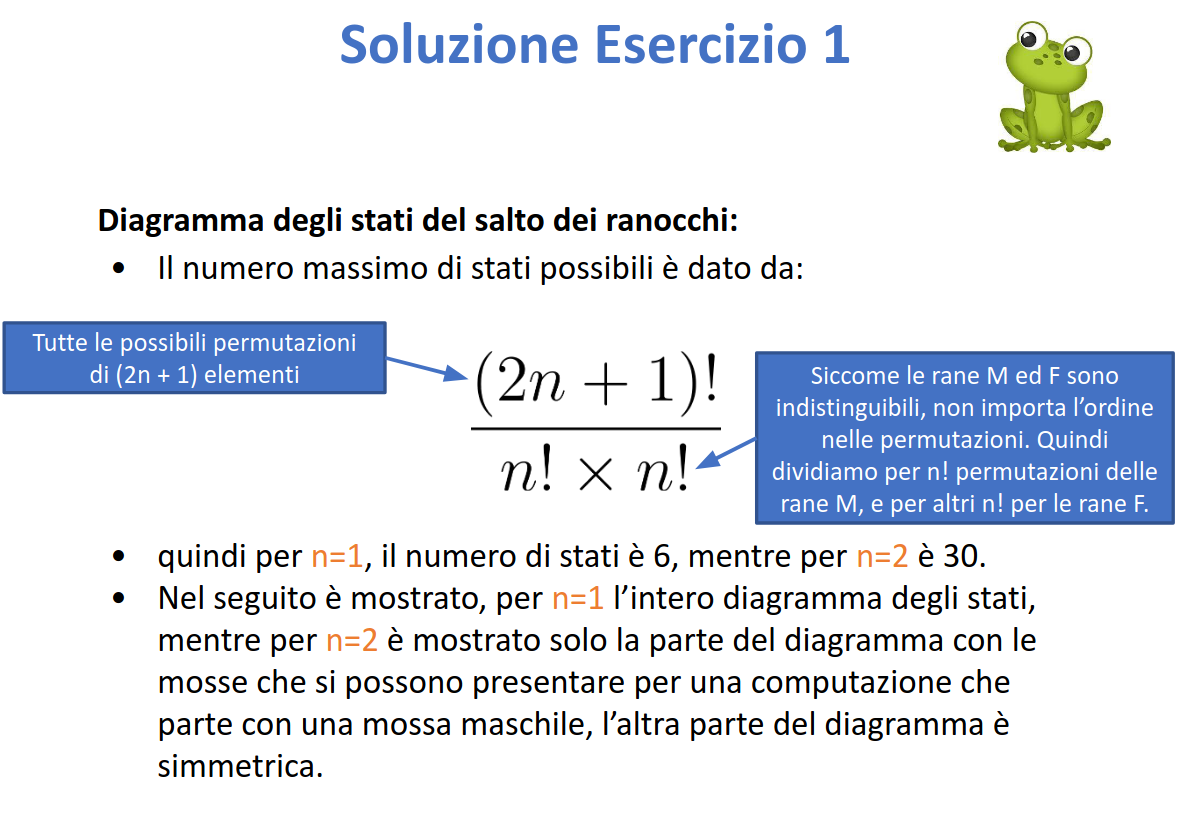
\includegraphics[scale=0.4]{01-IntroduzioneAllaProgrammazioneConcorrente/s1-1.png}
\end{center}

\begin{center}
    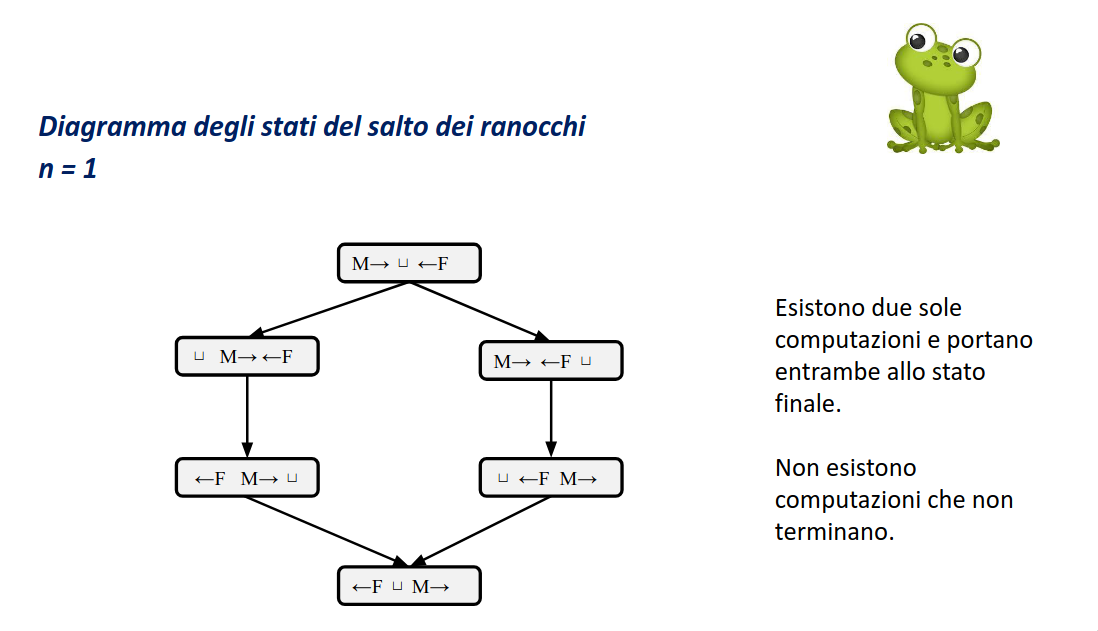
\includegraphics[scale=0.45]{01-IntroduzioneAllaProgrammazioneConcorrente/s1-2.png}
\end{center}

\begin{center}
    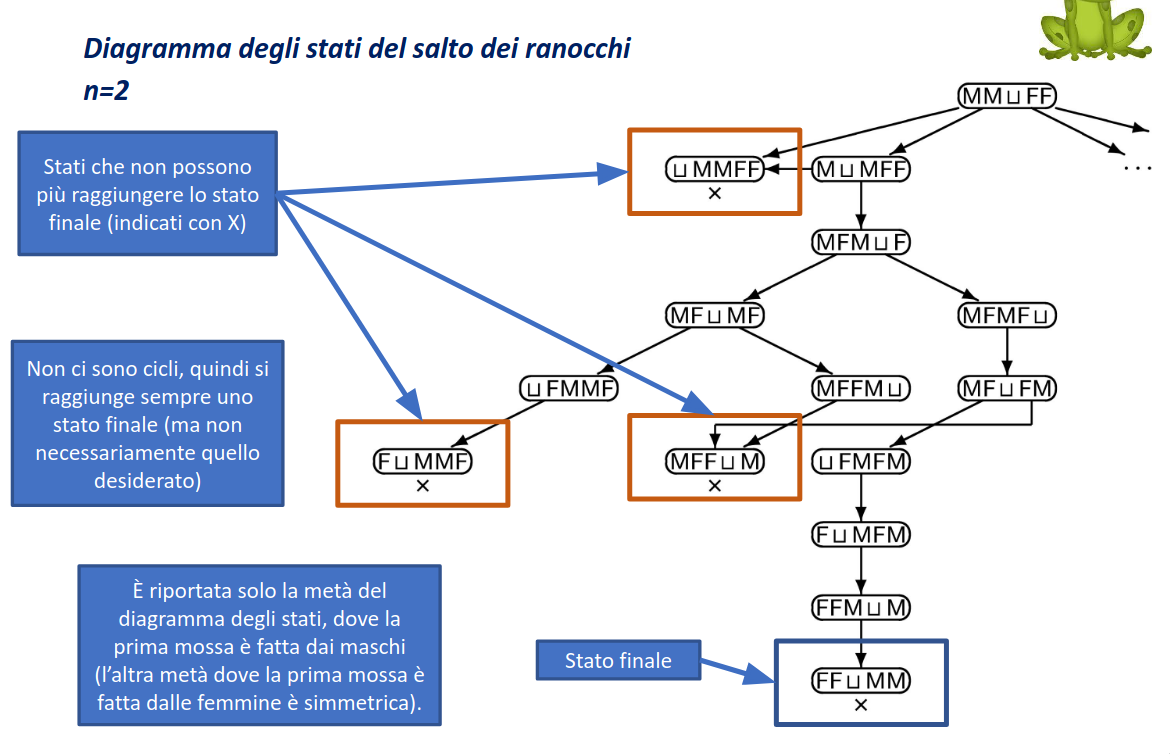
\includegraphics[scale=0.4]{01-IntroduzioneAllaProgrammazioneConcorrente/s1-3.png}
\end{center}

\begin{center}
    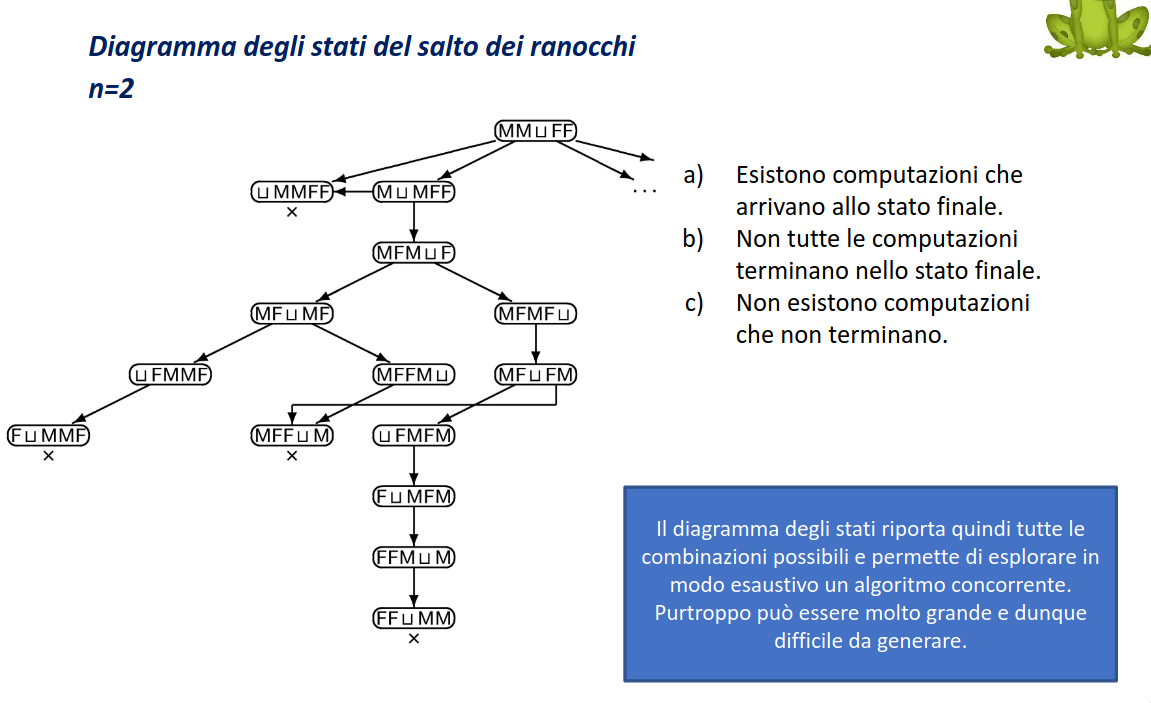
\includegraphics[scale=0.4]{01-IntroduzioneAllaProgrammazioneConcorrente/s1-4.png}
\end{center}
\pagebreak
\section{Conteggio Concorrente}

\begin{center}
    \centering
    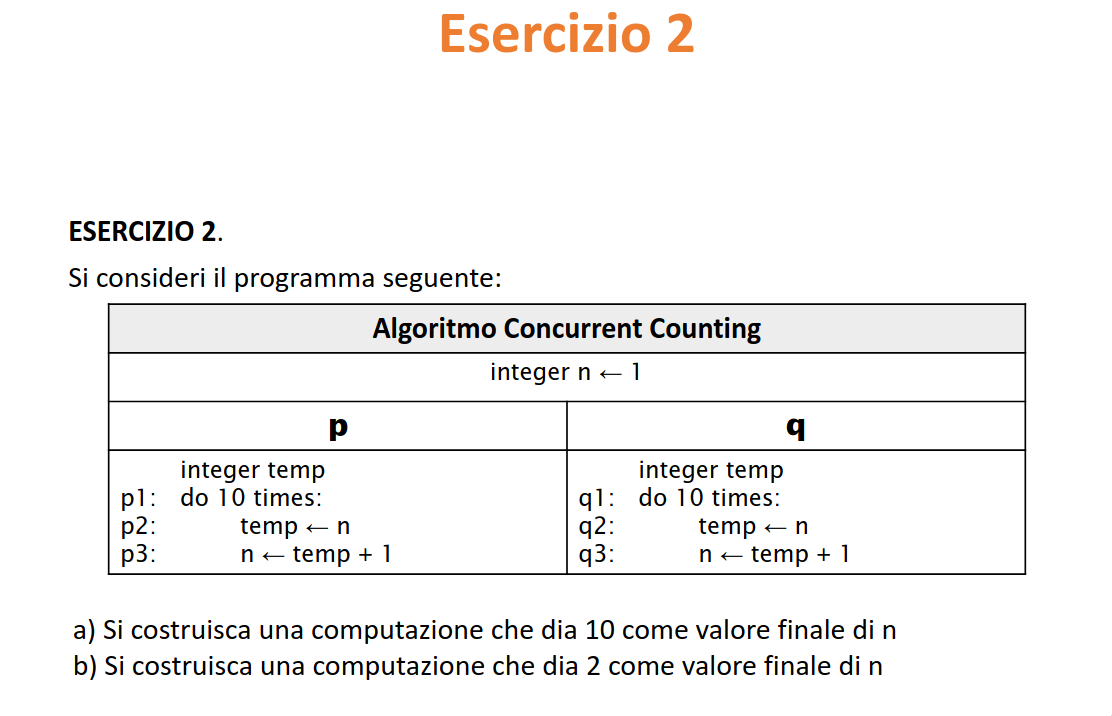
\includegraphics[scale=0.4]{01-IntroduzioneAllaProgrammazioneConcorrente/2-1.png}
  \end{center}

